\chapter{پیشگفتار}
%maybe use Zhang book ch1 intro
{\mmm{تقطیع تصاویر}{image segmentation}}
یکی از گام‌های مهم و اساسی در بسیاری از کاربردهای پردازش تصویر، ویدئو و بینایی ماشین است که اغلب به منظور تفکیک تصویر به ناحیه‌های مجزایی که در حالت ایده آل مشخص کننده اشیای مختلف در جهان واقعی هستند به کار می‌رود.
انجام صحیح این فرایند، تاثیر بسزایی بر کارایی الگوریتم‌های کاوش محتوا و ادراک تصاویر خواهد داشت.

مسئله تقطیع تصاویر، یکی از مسائل کلاسیک مطرح در حوزه بینایی ماشین است.
اما گذشته از اینکه ادراک انسان‌ها از تصاویر یکسان نبوده و دارای ابهام می‌باشد، از دیدگاه آماری نیز، این موضوع به دلایل زیر یک مسئله ذاتا مبهم به شمار می‌رود%
~\cite{yang_unsupervised_2008}:

\begin{itemize}
\item
خواص آماری ویژگیهای محلی مانند رنگ،
{\mmm{بافت}{texture}}،
لبه‌ها و
{\mmm{پیرامون}{contour}}
در تصاویر طبیعی، به طور معمول در مقیاس مکانی یا تفکیک‌پذیری یکسان، از همگنی یا برجستگی متفاوتی برخوردارند.
	این موضوع علاوه بر اینکه در میان چند تصویر مختلف قابل مشاهده است، در نواحی مختلف در یک تصویر نیز دیده می‌شود.
	بنابراین نباید انتظار داشت که نتیجه تقطیع یکتا باشد و می‌بایست یک ساختار سلسله مراتبی از تقطیع در مقیاس‌های مختلف را در نظر گرفت.
\item 
	گذشته از تغییرات بیان شده، امکان دارد که نواحی یا بافت‌های مختلف موجود در تصویر پیچیدگی‌های ذاتی متفاوتی داشته باشند که مسئله تعیین قطعات و تعداد آنها و درنتیجه ابعاد مدل آماری را به یک مسئله سخت تبدیل می‌نماید.
	به عنوان مثال اگر ما از توزیع گوسی برای مدل کردن ویژگیهای بافت‌های مختلف تصویر استفاده کنیم، قطعا این توزیع برای یک بافت پیچیده ابعاد بیشتری نسبت به یک بافت ساده خواهد داشت.
\end{itemize}

روش‌های زیادی برای تقطیع تصاویر و تفوق بر پیچیدگیهای اشاره شده پیشنهاد شده است که در فصل
\ref{ch:imageSegmentation}
به خلاصه‌ای از آنها اشاره خواهد شد.
اما در سالهای اخیر ایده‌ای که اولین بار توسط
\lr{Barlow}%
~\cite{barlow_possible_1961}
پیشنهاد شد، مورد توجه بیشتری قرار گرفته است.
او این فرضیه را بیان کرد که یکی از قاعده‌های اصلی سازمان‌دهی سیستم‌های سنسوری، کاهش
{\mmm{افزونگی}{redundancy}}
آماری موجود در بازنمایی ورودی‌های سنسوری است.
%from "Face Image Analysis by Unsupervised Learning" By Marian Stewart Bartlett, p8
به این معنا که اطلاعات مربوط به الگوها و نظم موجود در تحریکات سنسوری، در افزونگی موجود در این داده‌ها قرار داشته و تحریکاتی که هیچ افزونگی نداشته باشند، از نویز تصادفی قابل تشخیص نیستند.
در این تئوری ادعا می‌شود که ادراک ساختارها با استفاده از کشف وابستگی‌های موجود در تحریکات انجام می‌شود.
به عنوان مثال مجموعه نقاط نمایش داده شده در سمت چپ شکل
\ref{fig.redundancy}
از یک توزیع یکنواخت دوبعدی نمونه‌برداری شده‌است و کاملا بدون ساختار به نظر می‌رسد.
در تصویر سمت راست، نیمی از نقاط از توزیع یکنواخت نمونه‌برداری شده و نیم دیگر با دوران همان نقاط به اندازه پنج درجه حول مرکز توزیع تولید شده است.
این وابستگی ساده میان جفت‌های نقاط موجب پیدایش یک ساختار قابل ادراک در تصویر شده است.

\begin{figure}[t]
	\begin{center}
		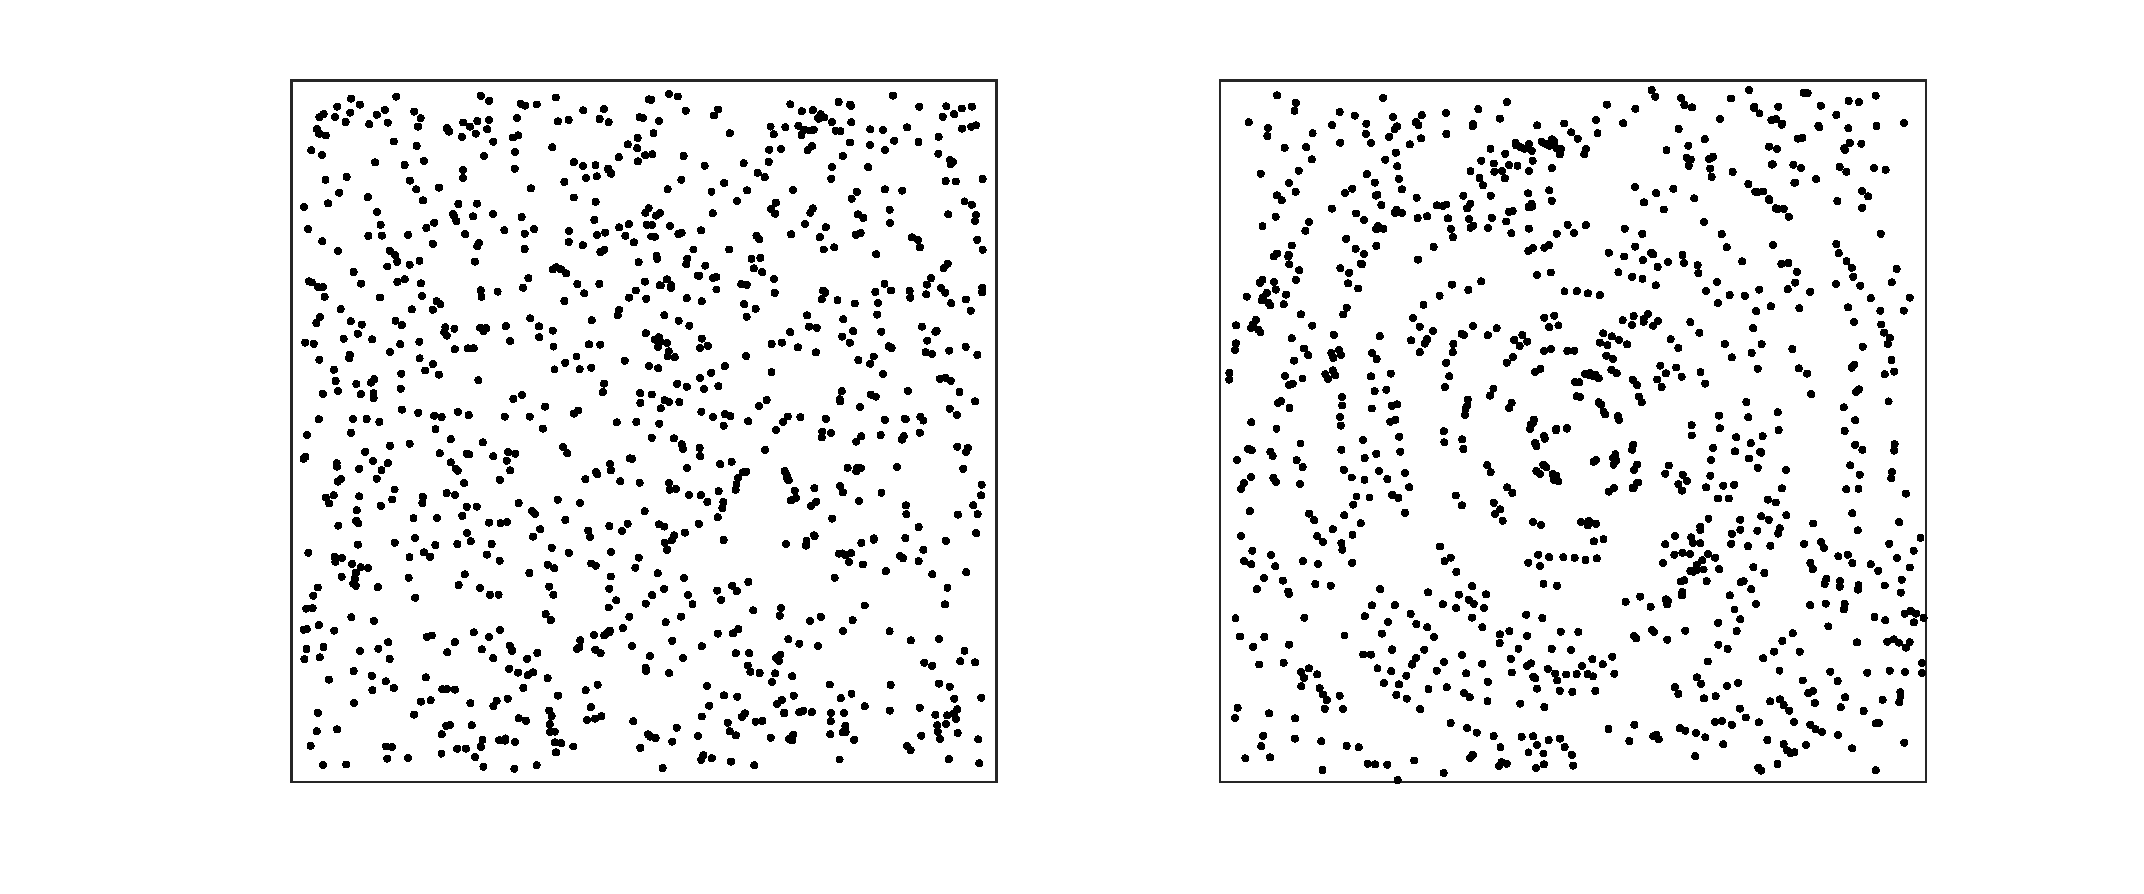
\includegraphics[width=\textwidth]{redundancy}
	\end{center}
\caption[مثالی از رابطه ادراک ساختار با افزونگی]
{
مثالی از رابطه ادراک ساختار با افزونگی -
\textbf{سمت چپ:}
مجموعه‌ای از نقاط نمونه‌برداری شده از یک توزیع یکنواخت دوبعدی.
\textbf{سمت راست:}
نیمی از نقاط از توزیع یکنواخت نمونه‌برداری شده و نیم دیگر با دوران همان نقاط به اندازه پنج درجه حول مرکز توزیع تولید شده است.
\label{fig.redundancy}
}
\end{figure}

به منظور استفاده از این تئوری در
{\mmm{یادگیری بدون نظارت}{unsupervised learning}}،
افزونگی مورد انتظار داده‌های ورودی، کد شده و از خروجی حذف می‌شود.
به این ترتیب، قابلیت اطمینان روش در شناسایی ساختارهای موجود در داده‌های جدید افزایش خواهد یافت.
یادگیری این تبدیل، معادل مدل کردن دانش پیشین در مورد وابستگی‌های آماری موجود در ورودی است%
\cite{barlow_possible_1961}.

در صنایع ارتباطی، کاهش افزونگی یک تکنیک مهم برای کمینه کردن بار ارسالی می‌باشد.
فرستنده پیام، پیش از اینکه پیام را ارسال نماید اطلاعات
{\mmm{افزونه}{redundant}}
موجود در آن را حذف می‌کند تا طول سیگنال کوتاه‌تر شده و با هزینه کمتر قابل ارسال باشد.
اما علاوه بر کاربرد فوق، کاهش افزونگی قابلیت این را دارد که ویژگی‌ها و الگو‌های بامعنی را از داده‌ها استخراج نماید.
به عنوان مثال در مبحث فشرده‌سازی زبان‌های طبیعی، یکی از اقداماتی که می‌توان به منظور ایجاد ویژگی‌های جدیـد انجام داد، ترکیب حروف الفبا و تولید نشانه‌های جدید می‌باشد.
بعضی از این نشانه‌ها احتمال وقوع بیشتری دارند که همان کلمات زبان مورد بررسی هستند.
بنابراین فشرده سازی متن می‌تواند موجب استخراج ویژگی‌های مفهومی مانند کلمات گردد.
در صورتی که این فرایند فشرده‌سازی را بیشتر ادامه دهیم ممکن است دریابیم که احتمال ترکیب بعضی کلمات با بعضی کلمات دیگر در جملات بیشتر است و در نتیجه ساختار جملات را کشف نماییم.

در مورد تصاویر نیز مسئله مشابه است و کاهش افزونگی می‌تواند موجب تشخیص ویژگی‌های جالب توجهی در تصویر گردد.
در این حالت الفبای مورد بررسی، شدت نور پیکسل‌های تصویر بوده و اقدامی که باید انجام شود این است که این پیکسل‌ها را به فضای دیگری تبدیل نماییم به طوری که نتایج از یکدیگر مستقل باشند.
برای مثال فرض شود که یک تصویر از کنار هم گذاشتن بافت‌هایی ساخته می‌شود که از هم مستقل هستند.
فضای پیکسلی تصویری در نتیجه می‌تواند به فضای بافتی تبدیل شود که در آن هر بافت با توجه به محل و اندازه و نوع آن مشخص می‌شود.
نوع بافت می‌تواند با یک مدل آماری مشخص شود.
محل و اندازه بافت با یک متغیر پنهان مشخص می‌شود که  مشخص می‌کند در یک بخش تصویر با چه احتمالی از یک بافت به بافت دیگر تغییر روی می‌دهد.

هدف از این پایان نامه، طراحی مدلی آماری برای تقطیع تصاویر دیجیتال از طریق کاهش افزونگی می‌باشد.
مدل ارائه شده می‌بایست توانایی مدل کردن ویژگی‌های آماری محلی تصاویر را داشته و بتوان با استفاده از استنتاج از متغیر پنهان ارائه شده توسط آن، مرزهای تقطیع تصویر را تعیین نمود.
برای این منظور از
{\mmm{مدل آمیخته}{mixture model}}ای از توزیع‌های
\lr{von Mises-Fisher}
استفاده شده است.
دلیل استفاده از مدل‌های آمیخته، ماهیت توزیع شدت نور پیکسل‌های تصاویر طبیعی در هر یک از بافت‌های موجود در تصویر است.
در تصاویر طبیعی معمولا هر بافت از تعدادی "زیربافت" در مقیاس کوچکتر تشکیل شده است%
~\cite{permuter_study_2006}.
به عنوان مثال می‌توان تصاویر هوایی گرفته شده از یک جنگل با انواع درختان مختلف را در نظر گرفت که بافت هر ناحیه از جنگل از ترکیب بافت‌های مربوط به درختان مختلف تشکیل شده است.
 بنابراین با توجه به این ویژگی، استفاده از مدل‌های آمیخته می‌تواند یک انتخاب مناسب برای مدل کردن بافت‌ها در تصاویر طبیعی باشد.
%TODO maybe use "Some Statistical Properties of Natural Images" from Dr thesis

یکی از دشواری‌های استفاده از مدل‌های آماری در کار با تصاویر طبیعی، مشکل ابعاد بالای پارامترهای مدل است که مشکلات زیادی را هنگام تخمین آن‌ها ایجاد می‌کند.
حتی برای پنجره‌های نسبتا کوچک انتخاب شده از این تصاویر نیز ابعاد پارامترهای مدل لازم برای بازنمایی داده‌ها می‌تواند به شدت بالا رفته و در تخمین چگالی مدل چالش ایجاد کند.
مدل
\lr{von Mises-Fisher}
با توجه به پایین بودن ابعاد پارامترهای آن، می‌تواند انتخاب خوبی برای اجزای مدل آمیخته باشد.


 در ادامه و در فصل
\ref{ch:mixtureModels}
نگاهی به مدل‌های آمیخته و مسائل و مشکلاتی که در عمل برای کار کردن با آن‌ها باید در نظر گرفته شوند خواهیم داشت.
سپس در فصل
\ref{ch:imageSegmentation}
به مرور مسئله تقطیع تصاویر و کارهای انجام شده در این حوزه می‌پردازیم.
همگام با پیشبرد این پروژه، یک بسته نرم‌افزاری جهت کار با مدل‌های آمیخته تهیه شده است که فصل
\ref{ch:mixest}
به معرفی آن اختصاص یافته است.
در فصل
\ref{ch:vMF}
با توزیع
\lr{von Mises-Fisher}
و مدل آمیخته متشکل از این نوع توزیع آشنا شده و الگوریتم پیشنهادی خود برای مقداردهی اولیه به پارامترهای این مدل را شرح خواهیم داد.
فصل
\ref{ch:proposedMethod}
به معرفی روش پیشنهاد شده برای تقطیع تصاویر پرداخته و در فصل
\ref{ch:results}
نتایج آزمایشات و مقایسه آن‌ها با برخی از الگوریتم های مطرح تقطیع تصاویر ارائه می‌شوند.
در انتها و در فصل
\ref{ch:conclusion}
به جمع‌بندی مطالب و بحث در مورد راه‌های ممکن برای بهبود نتایج می‌پردازیم.







